% Appendix A
\chapter{Additional Figures}

\newpage

\section{Scatterplot of all the variables} % Main appendix title

\label{AppendixA} % For referencing this appendix elsewhere, use \ref{AppendixA}

\lhead{Appendix A.1 \emph{Scatterplot of all the variables}} % This is for the header on each page - perhaps a shortened title
\begin{figure}[htbp]%
	\centering
		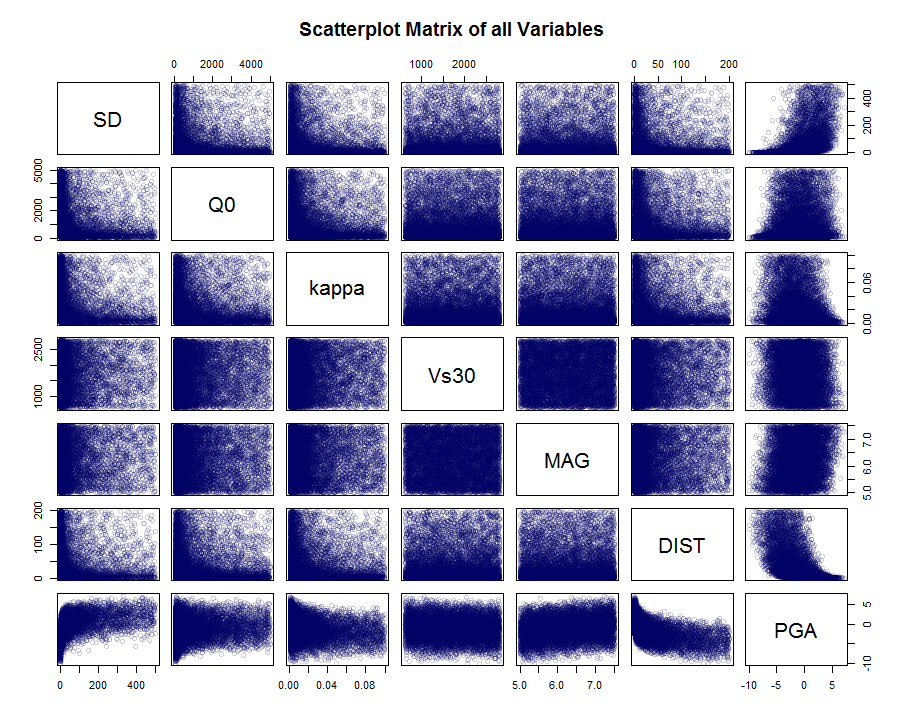
\includegraphics[angle=90,scale=0.45]{Figures/allvsall.pdf}
		\rule{35em}{0.5pt}
	\caption*{Scatterplot of all the variables}
\end{figure}

\newpage

\section{Folds of Learned Networks: Hill-Climber} % Main appendix title

\label{AppendixB} % For referencing this appendix elsewhere, use \ref{AppendixA}

\lhead{Appendix A.2 \emph{Folds of Learned Networks: Hill-Climber}} % This is for the header on each page - perhaps a shortened title
\begin{figure}[!htbp]%
	\centering
		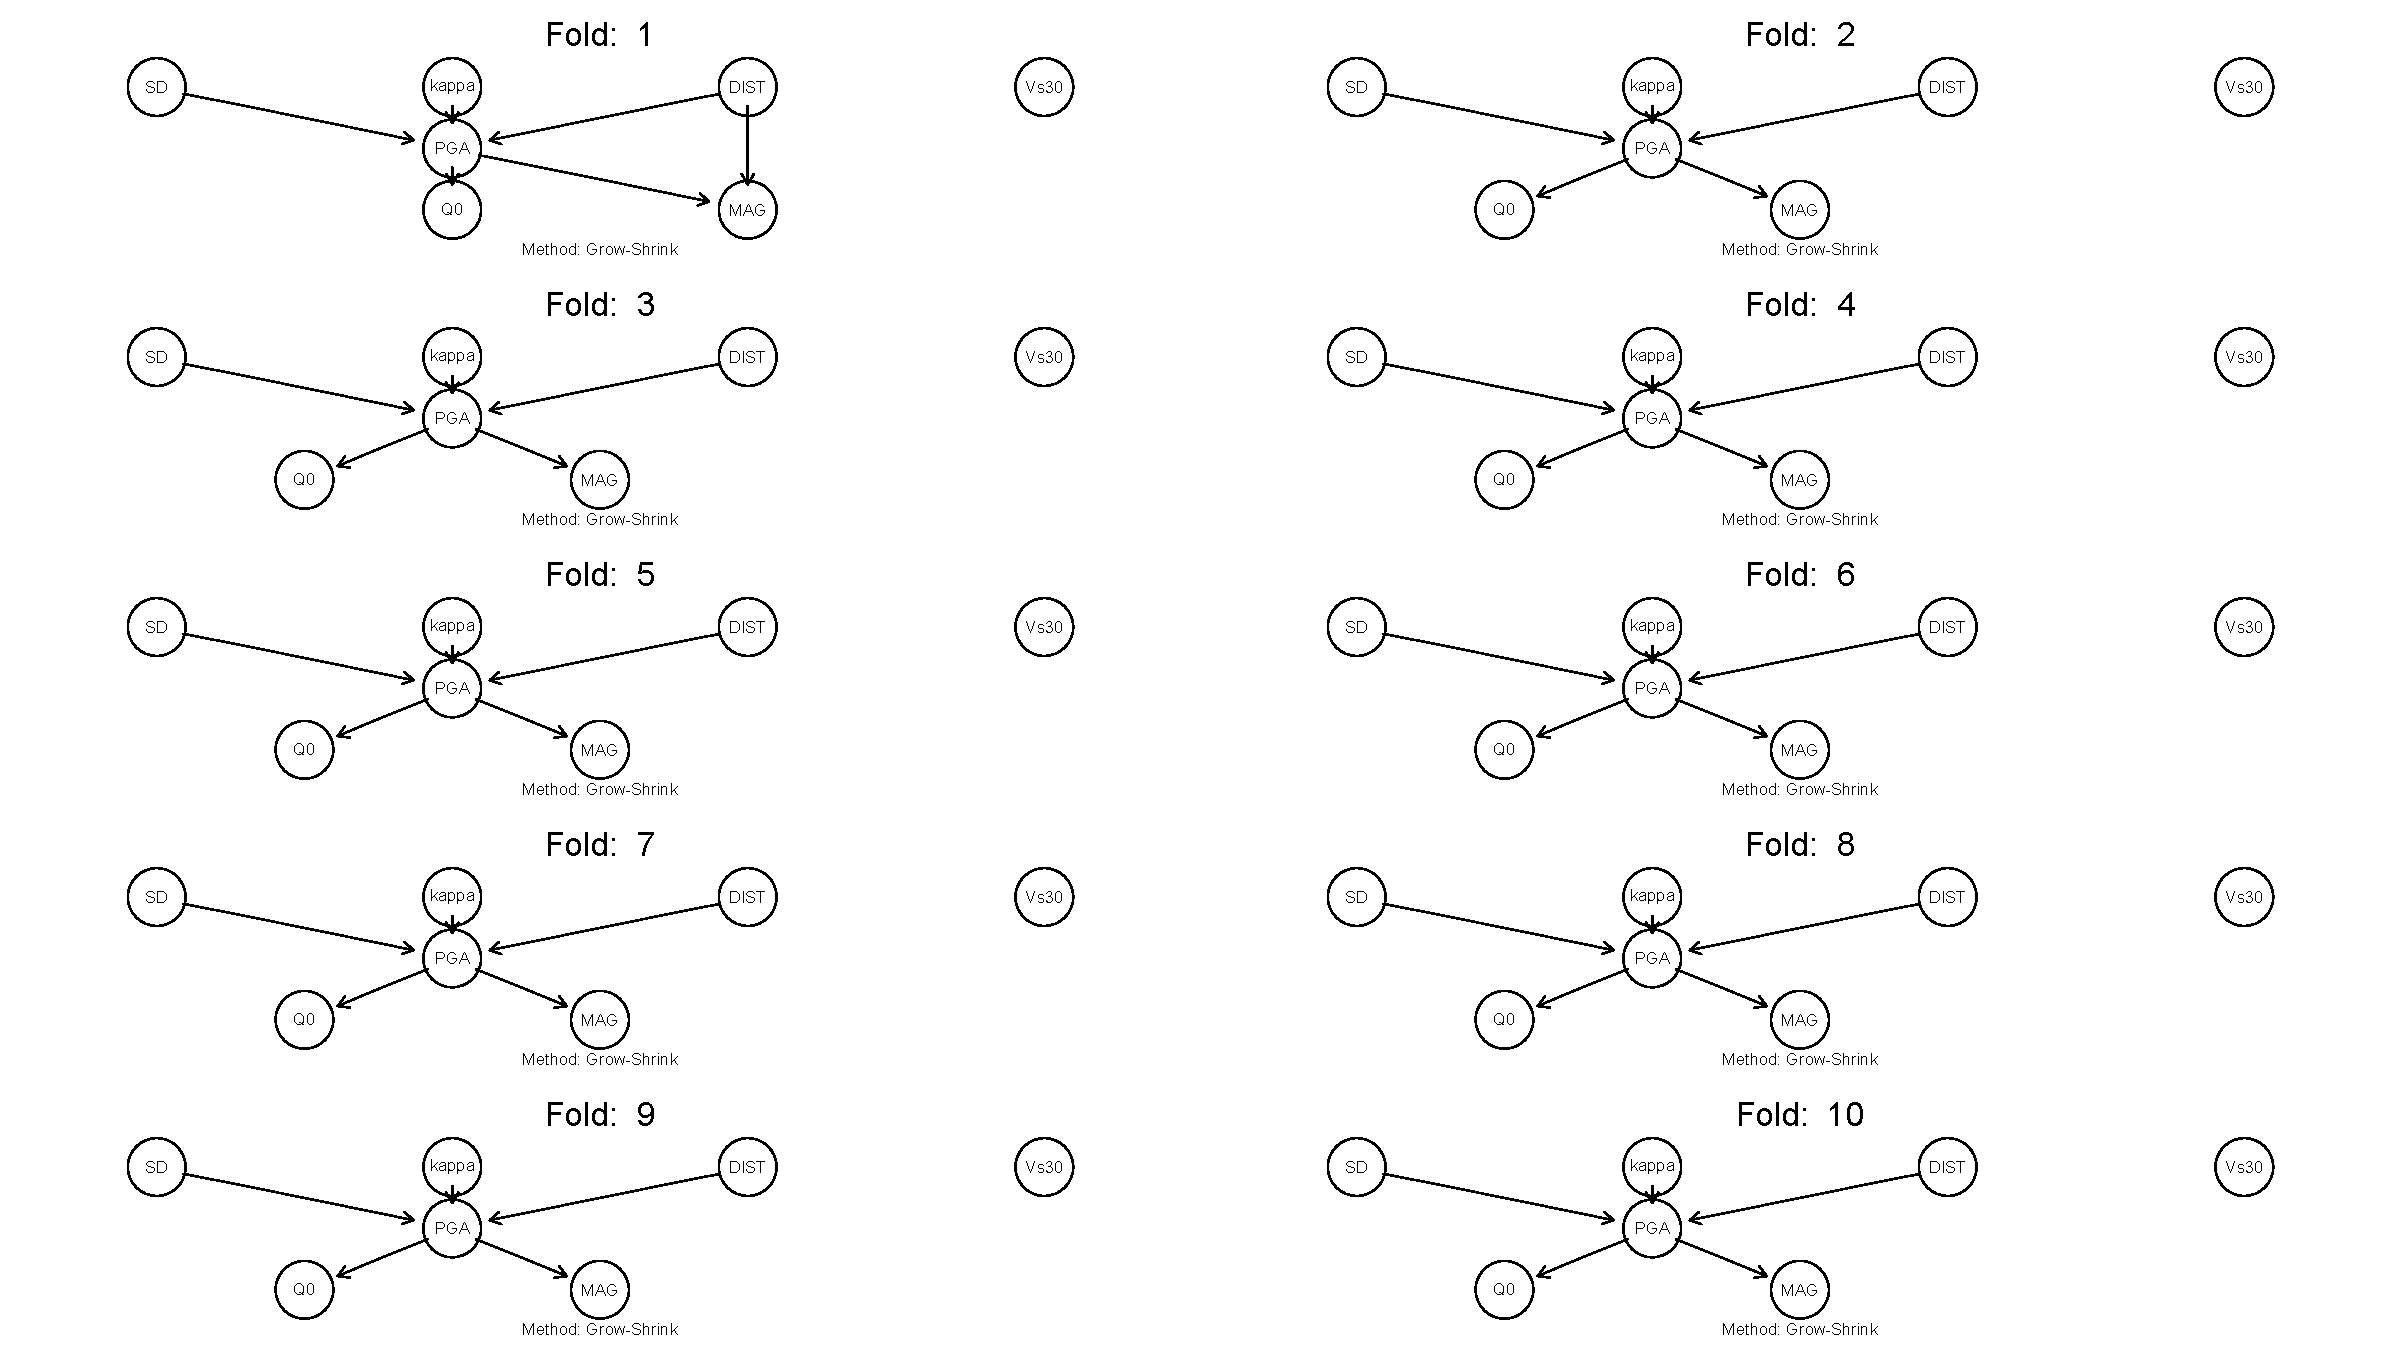
\includegraphics[angle=90,scale = 0.5]{Figures/hc.pdf}
		\rule{35em}{0.5pt}
	\caption*{Folds of Learned Networks: Hill-Climber}
\end{figure}

\newpage
\section{Folds of Learned Networks: Grow-Shrink} % Main appendix title

\label{AppendixC} % For referencing this appendix elsewhere, use \ref{AppendixA}

\lhead{Appendix A.3 \emph{Folds of Learned Networks: Grow-Shrink}} % This is for the header on each page - perhaps a shortened title
\begin{figure}[!htbp]%
	\centering
		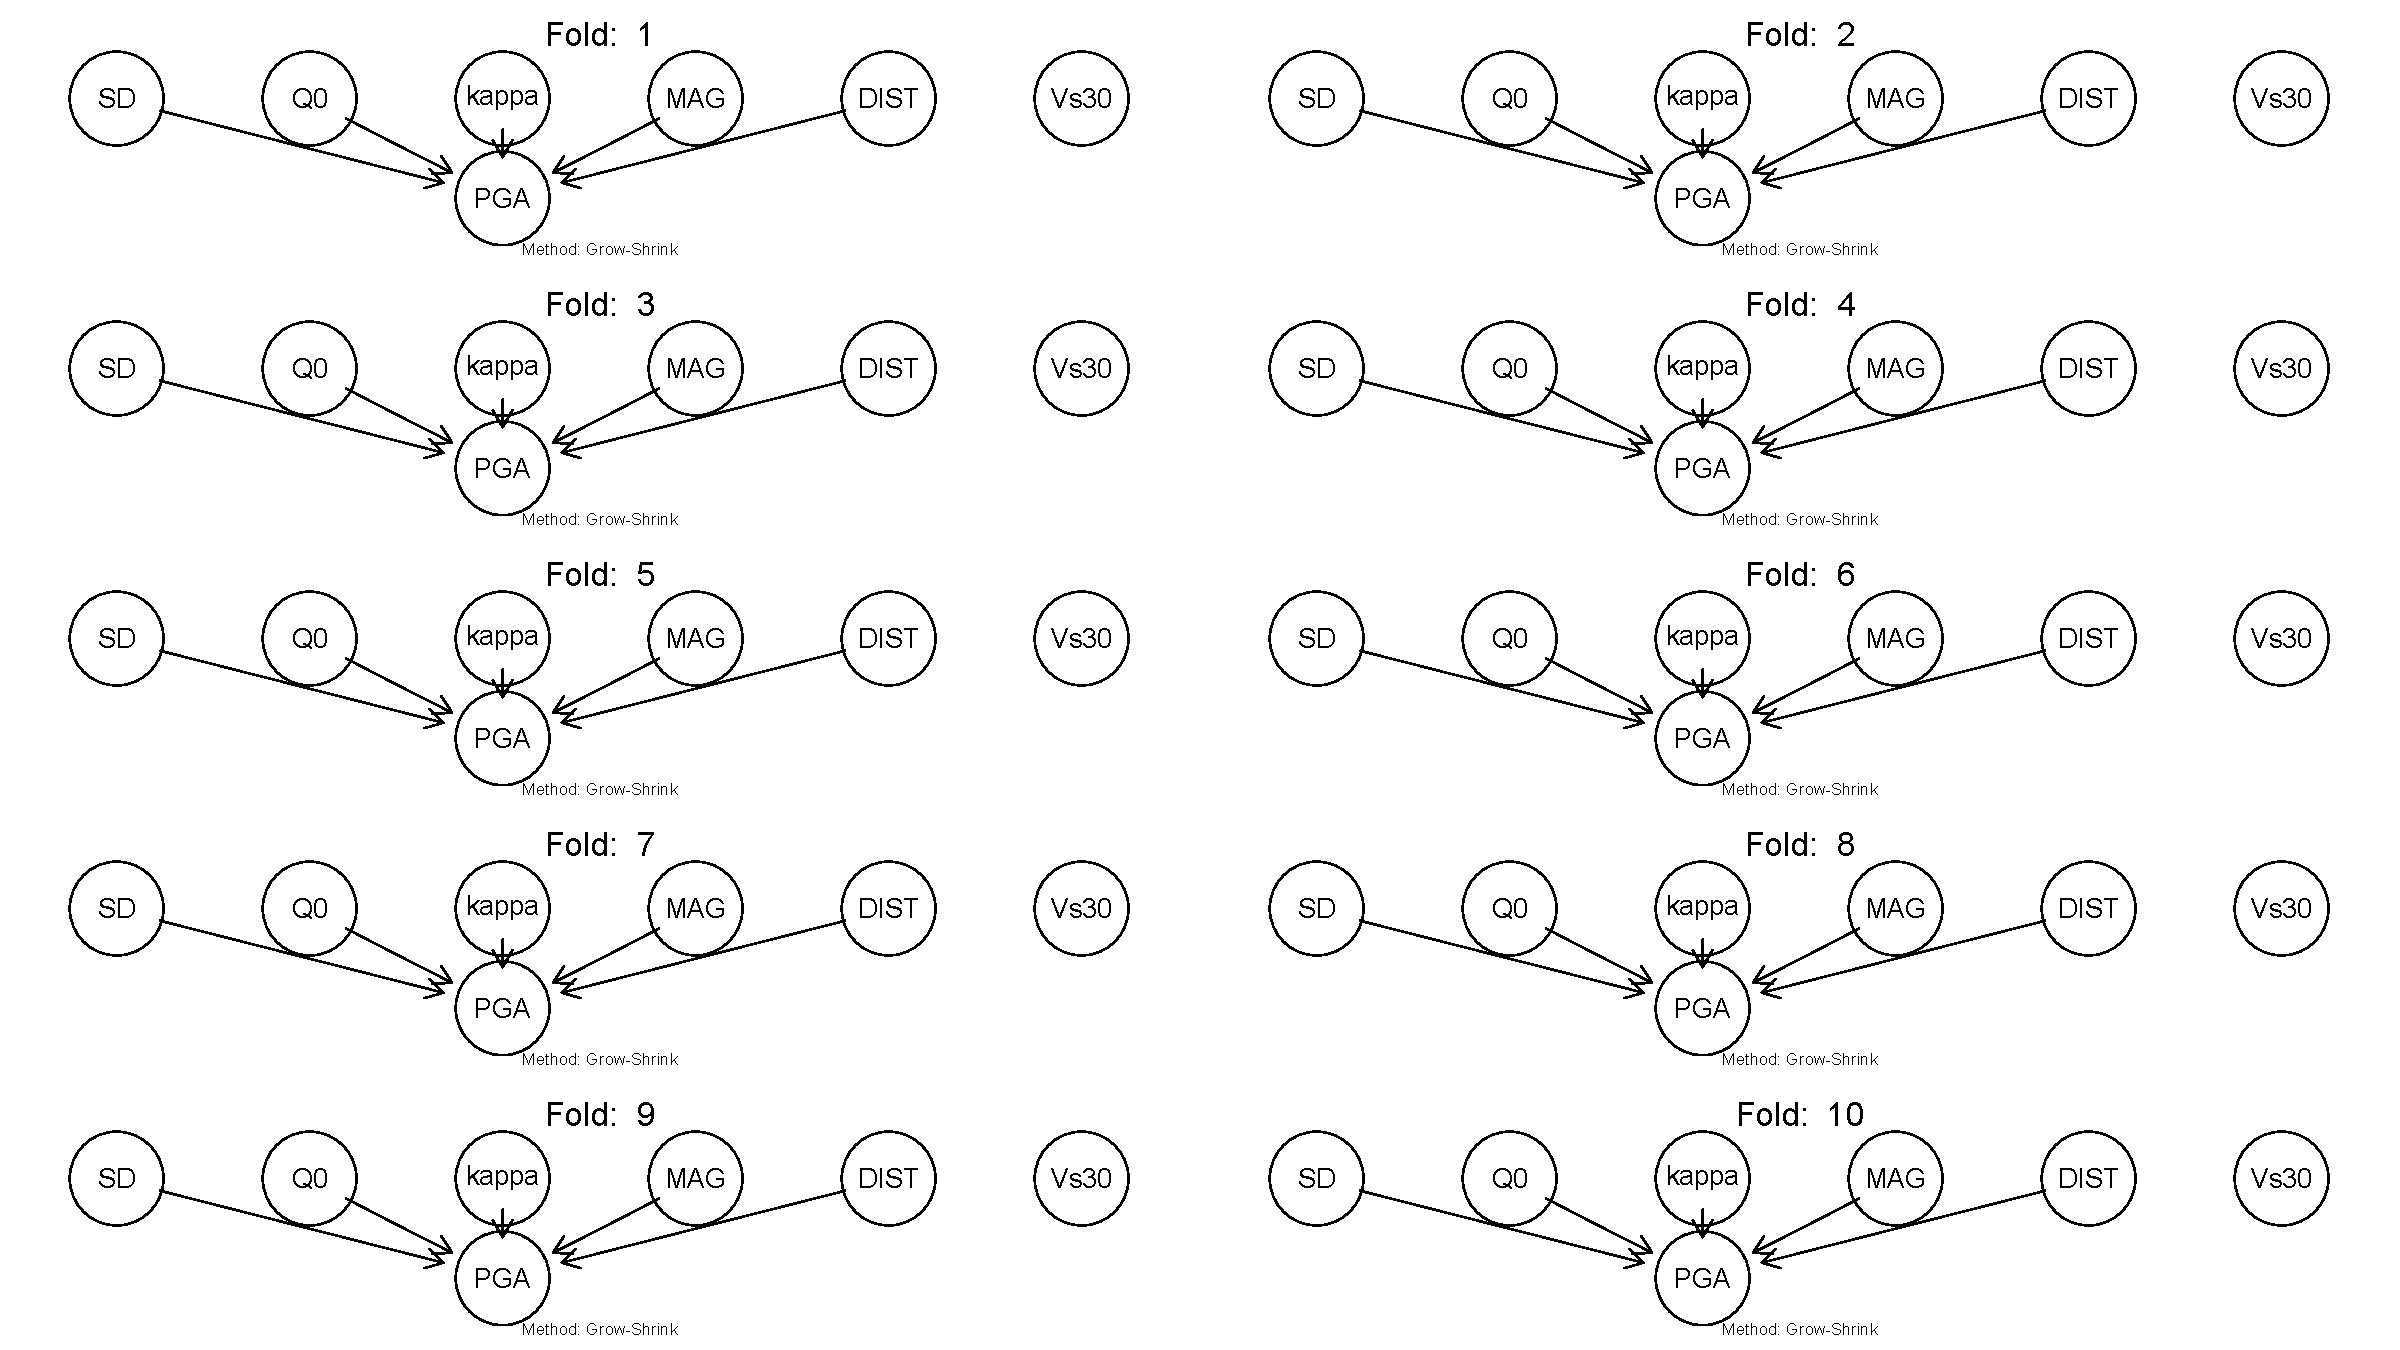
\includegraphics[angle=90,scale=0.5]{Figures/gs.pdf}
		\rule{35em}{0.5pt}
	\caption*{Folds of Learned Networks: Grow-Shrink}
\end{figure}